%-------------------------------------------------------------------------
% instructions.tex
%-------------------------------------------------------------------------

%-------------------------------------------------------------------------
\setjobnamebeamerversion{instructionsSlide}

\usetheme{Enib}
%-------------------------------------------------------------------------

%-------------------------------------------------------------------------
\newtheorem{rem}{Remarque}[section]
\newtheorem{defin}{Définition}[section]
\newtheorem{td}{\color{blue}TD}[section]
%-------------------------------------------------------------------------

%-------------------------------------------------------------------------
\lstset
{
language=Python,
basicstyle=\ttfamily,
identifierstyle=\ttfamily,
keywordstyle=\color{blue}\ttfamily,
commentstyle=\color{gray}\ttfamily,
stringstyle=\color{green}\ttfamily,
showstringspaces=false,
extendedchars=true,
numbers=left, 
numberstyle=\tiny,
frame=lines,
linewidth=0.95\textwidth,
xleftmargin=5mm
} 
%-------------------------------------------------------------------------

%-------------------------------------------------------------------------
\def\exo#1{\mbox{}\ \hfill\mbox{\color{blue}$\rule{2mm}{2mm}\,$\footnotesize\sc TD\ref{#1}}}
\def\exercice#1#2{\mbox{}\ \ TD \ref{#1}\ #2\ \dotfill\ \pageref{#1}\mbox{}}

\newenvironment{py}[1]{\begin{minipage}[t]{#1}\footnotesize}{\end{minipage}}
%-------------------------------------------------------------------------

\graphicspath{{../../fig/}}


%-------------------------------------------------------------------------
\title[Algorithmique]{\bf Initiation à l'algorithmique}
\subtitle{\bf --- instructions de base ---}

\author[\tt jacques.tisseau@enib.fr]{\large\bf Jacques TISSEAU}
\institute[\enib]{{\large\enib--\cerv}}
\date[enib\copyright 2009-2014]{\footnotesize enib\copyright 2009-2014}
%-------------------------------------------------------------------------

%-------------------------------------------------------------------------
\begin{document}
%-------------------------------------------------------------------------

%------------------------------------------
\begin{frame}
\frametitle{\uppercase{Informatique \hfill {S1}}}
%------------------------------------------
\titlepage

\end{frame}
\note{
\mbox{}\null\vfill

\begin{rem}[Notes de cours : couverture]
Ce support de cours accompagne le 
chapitre 2 des notes de cours \og Initiation à l'algorithmique\fg.
$$\fbox{
\includegraphics[width=10cm,page=1]{../../../pdf/cours/info-S1.pdf}}$$
\end{rem}
}
%------------------------------------------

%------------------------------------------
\begin{frame}
\frametitle{\uppercase{Instructions}}
\framesubtitle{\uppercase{Définitions}}
%------------------------------------------
\begin{block}{Instruction}
Commande élémentaire interprétée et exécutée par le processeur.
\end{block}
%\pause
\begin{block}{Jeu d'instructions}
Dans un processeur, ensemble des instructions que cette puce peut exécuter.
\end{block}
%\pause
\begin{block}{Bloc d'instructions}
Dans un algorithme, séquence d'instructions pouvant être vue
comme une seule instruction.
\end{block}
\end{frame}
\note{
\mbox{}\null\vfill

\begin{rem}[Cycles per Instruction]
Le c\oe ur du microprocesseur est régulé par un quartz qui 
oscille avec une fréquence exprimée en Hz.
Le temps de cycle est l'inverse de la fréquence.
Ainsi pour une fréquence de 100 MHz, on a un temps de cycle de 10 ns.
L'exécution d'une instruction nécessite plusieurs temps de cycle, 
c'est ce que l'on appelle le {\sc cpi} {\em(Cycles per Instruction)}.
\end{rem}
}
%------------------------------------------


%------------------------------------------
\begin{frame}
\frametitle{\uppercase{Jeux d'instructions}}
\framesubtitle{\uppercase{Définitions}}
%------------------------------------------
\begin{columns}[T]
\column{5.25cm}

\begin{block}{Classes d'instructions $\mu P$}
\begin{description}
\item[arithmétique :] {\tt +}, {\tt -}, {\tt *}, {\tt /}
\item[logique :\ \ \ \ \ ] {\tt not}, {\tt and}, {\tt or}
\item[transferts de données :] {\tt load}, {\tt store}, {\tt move}
\item[contrôle du flux d'instructions :] branchements, boucles, appels de procédure
\item[entrée-sortie :] {\tt read}, {\tt write}
\end{description}
\end{block}

%\pause
\column{5.25cm}

\begin{block}{Traitement des instructions}
\begin{enumerate}
\item {\tt fetch} : chargement de l'instruction,
\item {\tt decode} : décodage,
\item {\tt load operand} : chargement des données,
\item {\tt execute} : exécution,
\item {\tt result write back} : mise à jour.
\end{enumerate}
\end{block}

\end{columns}

\end{frame}
\note{
\mbox{}\null\vfill

\begin{rem}[Types d'architecture de micro-processeur]
\begin{itemize}
\item les architectures {\sc risc} {\em (Reduced Instruction Set Computer)}
	préconisent un petit nombre d'instructions élémentaires dans un format
	fixe;
\item les architectures {\sc cisc} {\em (Complex Instruction Set Computer)}
	sont basées sur des jeux d'instructions très riches de taille variable
	offrant des instructions composées de plus haut niveau d'abstraction.
\end{itemize}
Chaque architecture possède ses avantages et ses inconvénients :
pour le {\sc risc} la complexité est reportée au niveau du compilateur,
pour le {\sc cisc} le décodage est plus pénalisant. 
En fait les machines {\sc cisc} se sont orientées vers une architecture {\sc
risc} où les instructions {\sc cisc} sont traduites en instructions 
{\sc risc} traitées par le coeur du processeur. 
\end{rem}
}
%------------------------------------------


%------------------------------------------
\begin{frame}
\frametitle{\uppercase{Instructions de base}}
\framesubtitle{\uppercase{Commentaire, ne rien faire, bloc}}
%------------------------------------------
\begin{block}{Instructions}
\begin{description}
\item[commentaire:] aide pour l'utilisateur humain.\vspace*{1mm}

	\framebox[6cm][l]{\tt \alert{\#} fin de ligne ignorée \alert{$\hookleftarrow$}}
%\pause
\item[instruction vide:] ne rien faire.\vspace*{1mm}

	\framebox[6cm][l]{\tt \alert{pass}}
%\pause
\item[bloc d'instructions:] regrouper plusieurs instructions en une seule.\vspace*{1mm}

	\framebox[6cm][l]{\begin{minipage}{5.5cm}
	$instruction 1$\\[1mm]
	\mbox{}\ \ \ $\displaystyle \left| \begin{array}{l}
	instruction 2.1\\
	...\\
	instruction 2.n
	\end{array}\right.$\\[1mm]
	$instruction 3$
	\end{minipage}}
	
	{\footnotesize\em noter l'\alert{indentation} du bloc d'instructions 2}
\end{description}
\end{block}

\end{frame}
\note{}
%------------------------------------------

%------------------------------------------
\begin{frame}
\frametitle{\uppercase{Instructions de base}}
\framesubtitle{\uppercase{Affectation, alternatives, itérations}}
%------------------------------------------
\begin{block}{Instructions}
\begin{description}
\item[affectation:] changer la valeur d'une variable.\vspace*{1mm}

\framebox[8cm][l]{\begin{minipage}{7.5cm}\tt
variable \alert{=} expression
\end{minipage}}
%\pause
\item[conditions:] exécuter une instruction sous condition.\vspace*{1mm}

\framebox[8cm][l]{\begin{minipage}{7.5cm}\tt
\alert{if} condition\alert{:} bloc\\
\ {\color{blue}[}\alert{elif} condition\alert{:} bloc{\color{blue}]*}\\
\ {\color{blue}[}\alert{else}\alert{:} bloc{\color{blue}]}
\end{minipage}}
%\pause
\item[itérations:] répéter plusieurs fois la même instruction.\vspace*{1mm}

\framebox[8cm][l]{\begin{minipage}{7.5cm}\tt
\alert{while} condition\alert{:} bloc
\end{minipage}}
%%\pause

\mbox{}

\framebox[8cm][l]{\begin{minipage}{7.5cm}\tt
\alert{for} element \alert{in} sequence\alert{:} bloc
\end{minipage}}
\end{description}

\end{block}

\end{frame}
\note{
}
%------------------------------------------


%------------------------------------------
\begin{frame}
\frametitle{\uppercase{Variables}}
\framesubtitle{\uppercase{Définitions}}
%------------------------------------------
\begin{block}{Définition}
Une variable est un objet informatique qui associe un nom à une valeur 
qui peut éventuellement varier au cours du temps\\
(\alert{une variable dénote une valeur}).
\end{block}
%\pause

\begin{block}{Nom d'une variable}
Le nom d'une variable est un identificateur aussi explicite que possible 
(\alert{exprimer le contenu sémantique de la variable}).
%\pause

Exemples : 
\tt \begin{tabular}[t]{|l|l|}
\hline
\alert{:-(} & \alert{:-)} \\
\hline
x & pression \\
y & angleRotation \\
z & altitude \\
\hline
\end{tabular}\hspace*{1cm}%\pause
\begin{tabular}[t]{|l|l|}
\hline
\alert{:-(} & \alert{:-)} \\
\hline
t & temps \\
u & masse \\
v & vitesse \\
\hline
\end{tabular}

\end{block}

\end{frame}
\note{
\mbox{}\null\vfill

\begin{rem}[Mots réservés en {\sc Python}]
\centerline{\begin{tabular}{lllll}
        and       & del       & for       & is        & raise \\
        assert    & elif      & from      & lambda    & return\\
        break     & else      & global    & not       & try\\
        class     & except    & if        & or        & while\\
        continue  & exec      & import    & pass      & with\\
        def       & finally   & in        & print     & yield
\end{tabular}}
\end{rem}
}
%------------------------------------------


%------------------------------------------
\begin{frame}
\frametitle{\uppercase{Variables}}
\framesubtitle{\uppercase{Règles lexicales}}
%------------------------------------------
\begin{block}{Règles lexicales}
\begin{itemize}
\item Un nom de variable est une séquence de lettres (a\ldots  z , A\ldots  Z) et de chiffres (0\ldots  9), 
	qui doit toujours commencer par une lettre.\\
	\alert{{\tt a2pique}}, \alert{{\tt jeanMartin}}, \alert{{\tt ieee754}}
%\pause
\item Pas de lettres accentuées, de cédilles, d'espaces, de
      	caractères spéciaux tels que {\tt \$}, {\tt \#}, {\tt @}, etc., 
      	à l'exception du caractère {\tt \_} (souligné).\\
	\alert{{\tt vitesse\_angulaire}}, \alert{{\tt element}}, \alert{{\tt ca\_marche}}
%\pause
\item La casse est significative : les caractères majuscules et minuscules sont distingués.\\
      	\alert{{\tt python}} $\neq$ \alert{{\tt Python}} $\neq$ \alert{{\tt PYTHON}}
\end{itemize}
\end{block}

\end{frame}
\note{}
%------------------------------------------


%------------------------------------------
\begin{frame}
\frametitle{\uppercase{Variables}}
\framesubtitle{\uppercase{Conventions lexicales}}
%------------------------------------------
\begin{block}{Conventions lexicales}
\begin{itemize}
\item {\em a priori}, n'utiliser que des lettres minuscules\\
	{\tt \begin{tabular}[t]{|l|l|}
	\hline
	\alert{:-(} & \alert{:-)} \\
	\hline
	Variable & variable \\
	\hline
	\end{tabular}}
%\pause
\item n'utiliser les majuscules qu'à l'intérieur du nom pour augmenter la lisibilité\\
	{\tt \begin{tabular}[t]{|l|l|}
	\hline
	\alert{:-(} & \alert{:-)} \\
	\hline
	programmepython & programmePython \\
	\hline
	\end{tabular}}
%\pause
\item nom de constante tout en majuscule\\
	{\tt \begin{tabular}[t]{|l|l|}
	\hline
	\alert{:-(} & \alert{:-)} \\
	\hline
	rouge  & ROUGE \\
	\hline
	\end{tabular}}
	
\end{itemize}
\end{block}

\end{frame}
\note{}
%------------------------------------------



%------------------------------------------
\begin{frame}
\frametitle{\uppercase{Affectation}}
\framesubtitle{\uppercase{Définition}}
%------------------------------------------
\begin{block}{Définition}
Opération qui attribue une valeur à une variable.

$$\framebox{\tt ... \alert{=} ...}$$
\end{block}
%\pause
\begin{block}{Valeur d'une constante}
$$\framebox{\tt variable \alert{=} constante}$$
\end{block}
%\pause
\begin{block}{Valeur d'une expression}
$$\framebox{\tt variable \alert{=} expression}$$
\end{block}

\end{frame}
\note{}
%------------------------------------------


%------------------------------------------
\begin{frame}
\frametitle{\uppercase{Affectation}}
\framesubtitle{\tt variable \alert{=} constante}
%------------------------------------------
\begin{block}{Valeur d'une constante}
$$\framebox{\tt variable \alert{=} constante}$$
\end{block}
%\pause
\begin{block}{Exemple : initialisations}
\tt booleen \alert{=} False\\%\pause
\tt entier \alert{=} 3\\%\pause
\tt reel \alert{=} 0.0\\%\pause
\tt chaine \alert{=} "salut"\\%\pause
autreChaine \alert{=} 'bonjour, comment ça va ?'\\%\pause
\tt tableau \alert{=} [5,2,9,3]\\%\pause
\tt matrice \alert{=} [[1,2],[6,7],[9,1]]
\end{block}

\end{frame}
\note{
\mbox{}\null\vfill

\begin{rem}[Types de base en \python]
\centerline{\begin{tabular}{lll}
type & nom & exemples \\
\hline
booléens & \tt bool & {\tt False}, {\tt True}\\
entiers  & \tt int  & \tt 3, -7\\
réels    & \tt float & \tt 3.14, 7.43e-3\\
chaînes  & \tt str & \tt 'salut', "l'eau"\\
n-uplets & \tt tuple & \tt 1,2,3\\
listes   & \tt list  & \tt [1,2,3] \\
dictionnaires & \tt dict & \tt \{'a':4, 'r':8\}
\end{tabular}}
\end{rem}
}
%------------------------------------------


%------------------------------------------
\begin{frame}
\frametitle{\uppercase{Affectation}}
\framesubtitle{\tt variable \alert{=} expression}
%------------------------------------------
\begin{block}{Valeur d'une expression}
$$\framebox{\tt variable \alert{=} expression}$$
On évalue d'abord l'expression puis on affecte sa valeur
à la variable.
\end{block}
%\pause
\begin{block}{Exemple : calculs}
\tt somme \alert{=} n*(n+1)/2\\%\pause
\tt delta \alert{=} b*b - 4*a*c
\end{block}

%\pause

\begin{block}{Exemple : échange de valeurs entre 2 variables}
\tt tmp \alert{=} x\\
\tt x \alert{=} y\\
\tt y \alert{=} tmp
\end{block}


\end{frame}
\note{
\mbox{}\null\vfill

\begin{rem}[Principales affectations en {\sc Python}]
	\centerline{\tt\begin{tabular}{lll}
	a = b  & & \\ 
	\hline	
	a += b & $\equiv$ & a = a + b \\
	a -= b & $\equiv$ & a = a - b \\	
	a *= b & $\equiv$ & a = a * b \\ 	
	a /= b & $\equiv$ & a = a / b \\ 	
	a \%= b & $\equiv$ & a = a \% b \\	
	a **= b& $\equiv$ & a = a ** b 	
	\end{tabular}}
	\end{rem}
}
%------------------------------------------


%------------------------------------------
\begin{frame}
\frametitle{\uppercase{Affectation}}
\framesubtitle{\tt variable \alert{=} expression}
%------------------------------------------
\begin{block}{Exemple : modification}
\tt i \alert{=} i + 1 \ \ \ \ \# incrémentation\\%\pause
\tt i \alert{=} i - 1 \ \ \ \ \# décrémentation\\%\pause
\tt q \alert{=} q/b
\end{block}

%\pause
\begin{block}{Attention !}
L'affectation est une opération typiquement informatique qui se distingue de
l'égalité mathématique.\\
%\pause
En mathématique une expression du type \alert{\tt i = i+1}
se réduit en \\ \alert{\tt 0 = 1} !

%\pause
En informatique, l'expression \alert{\tt i = i+1}
conduit à ajouter \alert{\tt 1} à la valeur de \alert{\tt i} (évaluation de 
l'expression \alert{\tt i+1}),
puis à donner cette nouvelle valeur à \alert{\tt i} (affectation).
\end{block}
\end{frame}
\note{
\mbox{}\null\vfill

\begin{td}[Permutation circulaire]
Effectuer une permutation circulaire droite entre les valeurs de 4 entiers $x$, $y$, $z$ et $t$.
\end{td}

\begin{td}[Séquences d'affectations]
Quelles sont les valeurs des variables $a$, $b$, $q$ et $r$ 
après les séquences d'affectations suivantes ?

\begin{minipage}[t]{4cm}
	\begin{enumerate}
	\item	
	\noindent{\footnotesize\tt
	\mbox{}\ \ a = 19\\
	\mbox{}\ \ b = 6\\
	\mbox{}\ \ q = 0\\
	\mbox{}\ \ r = a\\
	\mbox{}\ \ r = r - b\\
	\mbox{}\ \ q = q + 1\\
	\mbox{}\ \ r = r - b\\
	\mbox{}\ \ q = q + 1\\
	\mbox{}\ \ r = r - b\\
	\mbox{}\ \ q = q + 1
	}
	\end{enumerate}
\end{minipage}
\hfill
\begin{minipage}[t]{4cm}
	\begin{enumerate}\setcounter{enumi}{1}
	\item	
	\noindent{\footnotesize\tt
	\mbox{}\ \ a = 12 \\
	\mbox{}\ \ b = 18 \\
	\mbox{}\ \ r = a\%b\\
	\mbox{}\ \ a = b \\
	\mbox{}\ \ b = r \\
	\mbox{}\ \ r = a\%b \\
	\mbox{}\ \ a = b \\
	\mbox{}\ \ b = r \\
	\mbox{}\ \ r = a\%b \\
	\mbox{}\ \ a = b \\
	\mbox{}\ \ b = r
	}
	\end{enumerate}
\end{minipage}
\end{td}
}
%------------------------------------------


%------------------------------------------
\begin{frame}
\frametitle{\uppercase{Alternatives}}
\framesubtitle{\uppercase{Instructions conditionnelles}}
%------------------------------------------
\begin{block}{Définition}
Exécuter une instruction sous condition.

$$\fbox{\begin{minipage}{7.5cm}\tt
\alert{if} condition\alert{:} bloc\\
\ {\color{blue}[}\alert{elif} condition\alert{:} bloc{\color{blue}]*}\\
\ {\color{blue}[}\alert{else}\alert{:} bloc{\color{blue}]}
\end{minipage}}$$

\begin{center}\footnotesize
Les instructions entre crochets ({\tt {\color{blue}[} ... {\color{blue}]}}) sont optionnelles.

\mbox{\tt{\color{blue}[} ... {\color{blue}]*}} signifie que les instructions entre crochets
peuvent être répétées 0 ou plusieurs fois.
\end{center}
\end{block}

Structure de contrôle effectuant un test et permettant un choix entre diverses 
parties du programme.
On sort ainsi de l'exécution purement séquentielle des instructions.
\end{frame}
\note{
\begin{rem}[Instructions conditionnelles]
$$\begin{tabular}{|l|l|}
\hline
%\multicolumn{2}{|c|}{Instructions conditionnelles}\\
%\hline
test simple         & {\begin{minipage}[t]{6cm}\tt if condition : blocIf \\ \mbox{} \end{minipage}} \\
\hline
alternative simple   & {\begin{minipage}[t]{6cm}\tt if condition : blocIf\\else: blocElse \\ \mbox{} \end{minipage}} \\
\hline
alternative multiple & {\begin{minipage}[t]{6cm}\tt if condition : blocIf\\elif condition1: blocElif1\\elif
condition2: blocElif2\\ \ldots \\else: blocElse \\ \mbox{} \end{minipage}}\\
\hline
\end{tabular}$$
\end{rem}
\mbox{}\null\vfill

\begin{td}[Opérateurs booléens dérivés]
En utilisant les opérateurs booléens de base ({\tt not}, {\tt and} et {\tt or}),
ecrire un algorithme qui affecte successivement à une variable {\tt s} 
le résultat des opérations booléennes suivantes :
ou exclusif ({\em xor}, $a \oplus b$), 
non ou ({\em nor}, $\overline{a+b}$), 
non et ({\em nand}, $\overline{a\cdot b}$), 
implication ($a \Rightarrow b$) et  
équivalence ($a \Leftrightarrow b$).
\end{td}
}
%------------------------------------------


%------------------------------------------
\begin{frame}
\frametitle{\uppercase{Alternatives}}
\framesubtitle{\uppercase{Test simple}}
%------------------------------------------
$$\fbox{\begin{minipage}{7.5cm}\tt
\alert{if} condition\alert{:} bloc
\end{minipage}}$$

\begin{columns}[T]

\column{5.25cm}

\begin{block}{Condition : comparaison}\tt

$$\begin{tabular}{ccc}
x & \alert{==} & y\\
x & \alert{!=} & y\\
x & \alert{\char`<}  & y\\
x & \alert{\char`<=} & y\\
x & \alert{>}  & y\\
x & \alert{>=} & y
\end{tabular}$$

\end{block}
%\pause

{\tt \alert{if} x < 0\alert{:} y = -x }\\%\pause
{\tt \alert{if} x != y\alert{:} y = x }
%\pause

\column{5.25cm}

\begin{block}{Condition : calcul booléen}\tt
$$\begin{tabular}{ccc}
  & \alert{not} & a\\
a & \alert{and} & b\\
a & \alert{or}  & b
\end{tabular}$$

\end{block}
%\pause

{\tt \alert{if} (x > 0) and (x < 2)\alert{:}\\
\mbox{}\ \ \ \ y = 3*x }\\%\pause
{\tt \alert{if} (x <= 0) or (x >= 2)\alert{:}\\
\mbox{}\ \ \ \ y = 4*x }

\end{columns}

\end{frame}
\note{
}
%------------------------------------------


%------------------------------------------
\begin{frame}
\frametitle{\uppercase{Alternatives}}
\framesubtitle{\uppercase{Alternative simple}}
%------------------------------------------
$$\fbox{\begin{minipage}{7.5cm}\tt
\alert{if} condition\alert{:} bloc\\
\alert{else}\alert{:} bloc
\end{minipage}}$$

\begin{columns}[T]

\column{5.25cm}
\begin{block}{Exemple : valeur absolue}
$$\begin{minipage}{5cm}\tt
\alert{if} x < 0\alert{:} \\
\mbox{}\ \ \ \ valeurAbsolue = -x\\%\pause
\alert{else:}  \\
\mbox{}\ \ \ \ valeurAbsolue = x
\end{minipage}$$
\end{block}
%\pause

\column{5.25cm}
\begin{block}{Exemple : maximum}
$$\begin{minipage}{5cm}\tt
\alert{if} x > y\alert{:}  \\
\mbox{}\ \ \ \ maximum = x\\%\pause
\alert{else:}  \\
\mbox{}\ \ \ \ maximum = y
\end{minipage}$$
\end{block}

\end{columns}

\end{frame}
\note{
{\bf Définitions}\begin{description}
\item[test simple] instruction de contrôle 
du flux d'instructions qui permet d'exécuter une instruction sous 
condition préalable.
\item[alternative simple] instruction 
de contrôle du flux d'instructions qui permet de choisir entre deux 
instructions selon qu'une condition est vérifiée ou non.
\end{description}
\null\vfill

\begin{td}[Alternative simple et test simple]
Montrer à l'aide d'un contre-exemple que l'alternative simple :\\
{\tt
\mbox{}\ \ if condition : blocIf\\
\mbox{}\ \ else : blocElse\\
}
n'est pas équivalente à la séquence de tests simples suivante :\\
{\tt
\mbox{}\ \ if condition : blocIf\\
\mbox{}\ \ if not condition : blocElse
}
\end{td}
}
%------------------------------------------


%------------------------------------------
\begin{frame}
\frametitle{\uppercase{Alternatives}}
\framesubtitle{\uppercase{Alternative simple}}
%------------------------------------------
Alternative simple
$$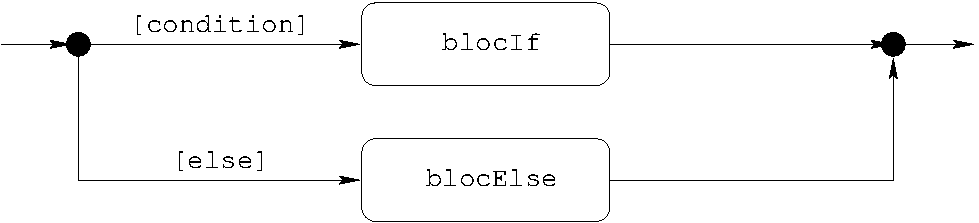
\includegraphics[width=9cm]{../fig/uml1.pdf}$$
\vspace*{5mm}

%\pause
Alternatives simples en cascade
$$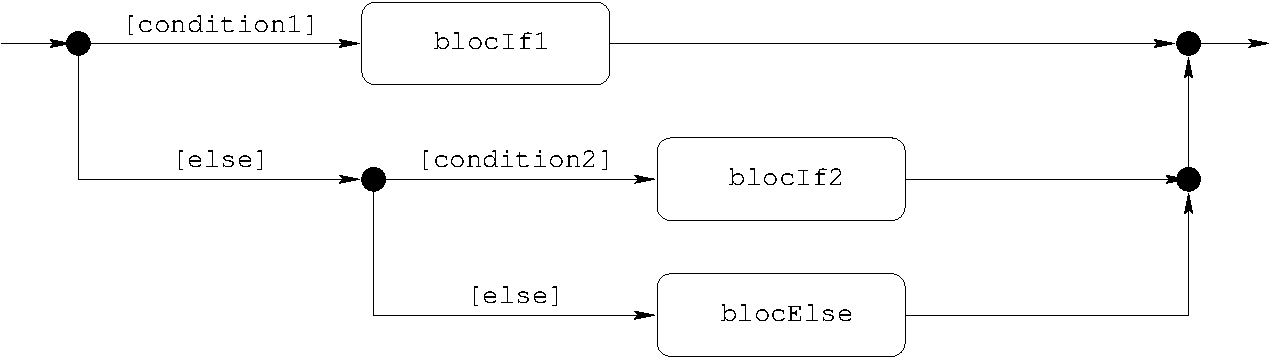
\includegraphics[width=9cm]{../fig/uml2.pdf}$$
\end{frame}
\note{
\begin{td}[Alternative simple]
Quelle est la valeur de la variable $y$ après la suite
	d'instructions suivante ?

	{\footnotesize\tt
	p = 1\\
	d = 0\\
	r = 0\\
	h = 1\\
	z = 0\\
	f = p and (d or r)\\
	g = not r \\
	m = not p and not z\\
	g = g and (d or h or m)\\
	if f or g : y = 1\\
	else : y = 0
	}
\end{td}

\begin{td}[Alternatives simples en cascade]
Quelle est la valeur de la variable $ok$ après la suite
	d'instructions suivante ?

	{\footnotesize\tt
	x = 2\\
	y = 3\\
	d = 5\\
	h = 4\\
	if x > 0 and x < d :\\
  	\mbox{}\ \ if y > 0 and y < h : ok = 1\\
	\mbox{}\ \ else : ok = 0\\
	else : ok = 0
	}
\end{td}
}
%------------------------------------------


%------------------------------------------
\begin{frame}
\frametitle{\uppercase{Alternatives}}
\framesubtitle{\uppercase{Alternatives multiples}}
%------------------------------------------
$$\fbox{\begin{minipage}{7.5cm}\tt
\alert{if} condition\alert{:} bloc\\
\alert{elif} condition\alert{:} bloc\\
\ldots\\
\alert{else}\alert{:} bloc
\end{minipage}}$$


\begin{block}{Exemple : mentions du bac}
$$\begin{minipage}{9cm}\tt
\alert{if} note < 10\alert{:} mention = "ajourné"\\%\pause
\alert{elif} note < 12\alert{:} mention = "passable"\\%\pause
\alert{elif} note < 14\alert{:} mention = "assez bien"\\%\pause
\alert{elif} note < 16\alert{:} mention = "bien"\\%\pause
\alert{else:} mention = "très bien"
\end{minipage}$$
\end{block}


\end{frame}
\note{
{\bf Définitions}\begin{description}
\item[alternative multiple] instruction de contrôle du flux d'instructions 
qui permet de choisir entre plusieurs instructions en cascadant des alternatives simples.
\end{description}
\null\vfill

\begin{td}[Alternatives multiples]
Quelle est la valeur de la variable $y$ après la suite
	d'instructions suivante ?

	{\footnotesize\tt
	x = 3\\
	y = -2\\
	if x < y : y = y - x\\
	elif x == y : y = 0\\
	else : y = x - y
	}
\end{td}
}
%------------------------------------------


%------------------------------------------
\begin{frame}
\frametitle{\uppercase{Alternatives}}
\framesubtitle{\uppercase{Alternatives multiples}}
%------------------------------------------
$$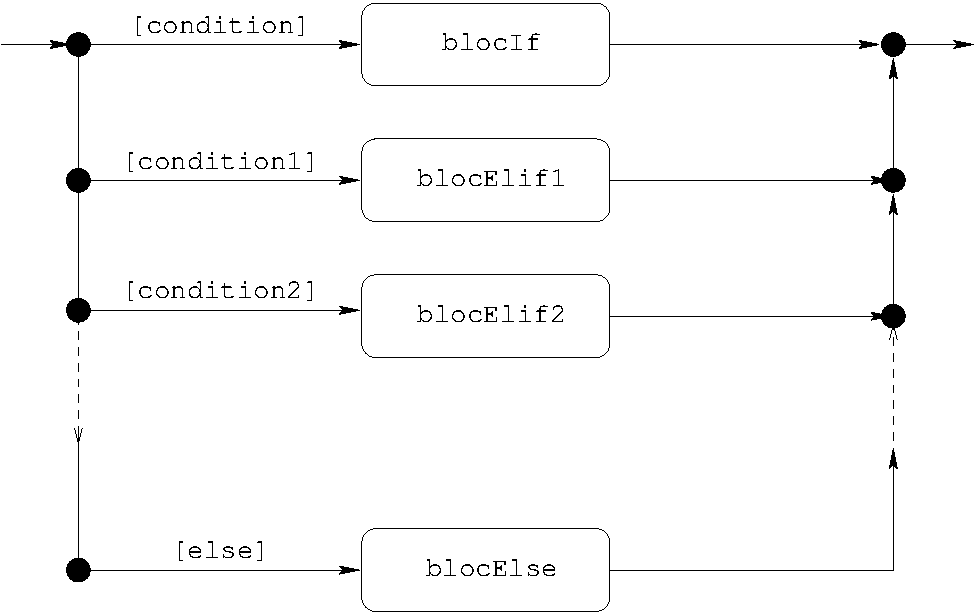
\includegraphics[width=9cm]{../fig/uml3.pdf}$$

\end{frame}
\note{
\mbox{}\null\vfill

\begin{td}[Prix d'une photocopie]
Ecrire un algorithme qui affiche le prix de n photocopies sachant que le reprographe facture 0,10 E les dix premières photocopies, 0,09 E les vingt suivantes et 0,08 E au-delà.
\end{td}

\begin{td}[Calcul des impôts]
Ecrire un algorithme qui affiche si un contribuable d'un pays imaginaire
	est imposable ou non sachant que :
	\begin{itemize}
	\item les hommes de plus de 18 ans paient l'impôt,
    	\item les femmes paient l'impôt si elles ont entre 18 et 35 ans,
	\item les autres ne paient pas d'impôt.
	\end{itemize}
\end{td}
}
%------------------------------------------


%------------------------------------------
\begin{frame}
\frametitle{\uppercase{Boucles}}
\framesubtitle{\uppercase{Instructions itératives}}
%------------------------------------------
\begin{block}{Définition}
Répétition d'un bloc d'instructions 0 ou plusieurs fois.

\color{blue}
$$\fbox{\begin{minipage}{9cm}\tt 
\alert{while} condition\alert{:} bloc
\end{minipage}}$$


$$\fbox{\begin{minipage}{9cm}\tt 
\alert{for} element \alert{in} sequence\alert{:} bloc
\end{minipage}}$$
\end{block}

Structures de contrôle destinées à être exécutées plusieurs fois 
(la structure de contrôle relançant l'exécution du bloc 
tant qu'une condition est remplie).

\end{frame}
\note{
\mbox{}\null\vfill

\begin{rem}[Instructions itératives]
$$\begin{tabular}{|l|l|}
\hline
itération conditionnelle & {\begin{minipage}[t]{6cm}\tt while condition : blocWhile \\ \mbox{} \end{minipage}} \\
\hline
parcours de séquence & {\begin{minipage}[t]{7cm}\tt for element in sequence : blocFor \\ \mbox{} \end{minipage}} \\
\hline
\end{tabular}$$
\end{rem}
}
%------------------------------------------



%------------------------------------------
\begin{frame}
\frametitle{\uppercase{Boucles}}
\framesubtitle{\uppercase{Itération conditionnelle}}
%------------------------------------------
\begin{block}{Boucle {\tt while}}
$$\fbox{\begin{minipage}{9cm}\tt 
\alert{while} condition\alert{:} bloc
\end{minipage}}$$
%\pause

\begin{itemize}
\item Le bloc d'instructions d'une boucle {\tt while} peut ne jamais être
exécuté (condition non vérifiée la première fois).

Exemple : 
	\begin{minipage}[t]{8cm}\tt 
	i = 0\\ 
	\alert{while} i > 0\alert{:} bloc 
	\end{minipage}

%\pause
\item On peut ne jamais sortir d'une boucle {\tt while}
(condition toujours vérifiée).

Exemple : {\tt \alert{while} True\alert{:} bloc }
\end{itemize}
\end{block}

\end{frame}
\note{
{\bf Définitions}\begin{description}
\item[itération conditionnelle] instruction de contrôle du flux d'instructions
qui permet sous condition préalable de répéter zéro ou plusieurs fois la même instruction.
\end{description}
\null\vfill

\begin{td}[Dessin d'étoiles]
Ecrire un algorithme itératif qui affiche les $n$ lignes suivantes (l'exemple
est donné ici pour $n=6$) : \\
\begin{minipage}[t]{2cm}\tt
******\\
*****\\
****\\
***\\
**\\
*
\end{minipage}
\hfill
\begin{minipage}[t]{3cm}
Rappel \python\ : \\
{\tt
\mbox{}\ \ \ \ >>> 5*'r'\\
\mbox{}\ \ \ \ 'rrrrr'\\
\mbox{}\ \ \ \ >>> 2*'to'\\
\mbox{}\ \ \ \ 'toto'
}
\end{minipage}
\end{td}
}
%------------------------------------------


%------------------------------------------
\begin{frame}
\frametitle{\uppercase{Itération conditionnelle}}
\framesubtitle{\uppercase{Elévation à la puissance}}
%------------------------------------------
$$p = x^n$$

\begin{columns}\tt
\column{5.25cm}
\fbox{\begin{minipage}{4.75cm}\color{blue}
x = 2\\
n = 3\\
i = 0\\
p = 1\\
{\color{black}print(x, n, p, i)}\\
\alert{while} i < n\alert{:} \\
\mbox{}\ \ p = p * x\\
\mbox{}\ \ i = i + 1\\
\mbox{}\ \ {\color{black}print(x, n, p, i)}\\
{\color{black}print(x, n, p, i)}
\end{minipage}}
%\pause

\column{5.25cm}
$$\begin{array}{|c|c|c|c|}
\hline
x & n & p & i\\
\hline
2 & 3 & 1 & 0\\\hline
%\pause
2 & 3 & 2 & 1\\%\pause
2 & 3 & 4 & 2\\%\pause
2 & 3 & 8 & 3\\\hline
%\pause
2 & 3 & 8 & 3\\
\hline
\end{array}$$
$$p = 8 = 2^3 = x^n$$
\end{columns}

\end{frame}
\note{
\mbox{}\null\vfill

\begin{td}[Fonction factorielle]
Ecrire un algorithme qui calcule $n! = 1\cdot 2\cdot 3\cdot \ldots \cdot (n-1)\cdot n$.
\end{td}
}
%------------------------------------------


%------------------------------------------
\begin{frame}
\frametitle{\uppercase{Itération conditionnelle}}
\framesubtitle{\uppercase{Division entière}}
%------------------------------------------
$$a = bq+r$$

\begin{columns}\tt
\column{5cm}
\fbox{\begin{minipage}{4.75cm}\color{blue}
a = 8\\
b = 3\\
q = 0\\
r = a\\
{\color{black}print(a, b, r, q)}\\
\alert{while} r >= b\alert{:}\\
\mbox{}\ \ r = r - b\\
\mbox{}\ \ q = q + 1\\
\mbox{}\ \ {\color{black}print(a, b, r, q)}\\
{\color{black}print(a, b, r, q)}
\end{minipage}}
%\pause

\column{5cm}
$$\begin{array}{|c|c|c|c|}
\hline
a & b & r & q\\
\hline
8 & 3 & 8 & 0\\\hline
%\pause
8 & 3 & 5 & 1\\%\pause
8 & 3 & 2 & 2\\\hline
%\pause
8 & 3 & 2 & 2\\
\hline
\end{array}$$
$$a = bq + r = 3\cdot 2 + 2 = 8$$
\end{columns}


\end{frame}
\note{
\mbox{}\null\vfill

\begin{td}[Pgcd de 2 entiers]
Ecrire un algorithme qui calcule le plus grand commun diviseur de 2 entiers $a$ et $b$ sachant que 
$${\rm pgcd}(a,b) = {\rm pgcd}(b,a\mbox{\tt\%}b) = \cdots = {\rm pgcd}(d,0) = d$$ 
\end{td}
}
%------------------------------------------


%------------------------------------------
\begin{frame}
\frametitle{\uppercase{Itération conditionnelle}}
\framesubtitle{\uppercase{Racine carrée entière}}
%------------------------------------------
$$r = \sqrt{n}$$

\begin{columns}\tt
\column{5cm}
\fbox{\begin{minipage}{4.75cm}\color{blue}
n = 17\\
r = 0\\
{\color{black}print(n, r)}\\
\alert{while} (r+1)**2 <= n\alert{:}\\
\mbox{}\ \ r = r + 1\\
\mbox{}\ \ {\color{black}print(n, r)}\\
{\color{black}print(n, r)}
\end{minipage}}
%\pause

\column{5cm}
$$\begin{array}{|c|c|}
\hline
n & r \\
\hline
17 & 0 \\\hline
%\pause
17 & 1 \\%\pause
17 & 2 \\%\pause
17 & 3 \\%\pause
17 & 4 \\\hline
%\pause
17 & 4 \\
\hline
\end{array}$$
$$r^2 = 4^2 = 16 \leq 17 = n$$
$$n = 17 < (r+1)^2 = 5^2 = 25$$
$$r^2 \leq n < (r+1)^2$$
\end{columns}

\end{frame}
\note{
\mbox{}\null\vfill

\begin{td}[Itérations conditionnelles]
\begin{enumerate}
\item Que fait cette suite d'instructions ?

	{\footnotesize\tt
	x = 0\\
	while x <= 0 or x > 5 :\\
	\mbox{}\ \ x = input('entrer un nombre : ')
	}
\item Quelle est la valeur de la variable $s$
	à la fin des instructions suivantes ?

	{\footnotesize\tt
	b = 2\\
	k = 8\\
	n = 23\\
	s = 0\\
	i = k - 1\\
	q = n\\
	while q != 0 and i >= 0 :\\
  	\mbox{}\ \ s = s + (q\%b)*b**(k-1-i)\\
  	\mbox{}\ \ print(q\%b,end=' ')\\
  	\mbox{}\ \ q = q/b\\
  	\mbox{}\ \ i = i - 1
	}
\end{enumerate}
\end{td}
}
%------------------------------------------


%------------------------------------------
\begin{frame}
\frametitle{\uppercase{Boucles}}
\framesubtitle{\uppercase{Itération conditionnelle}}
%------------------------------------------
Boucle {\tt while}
$$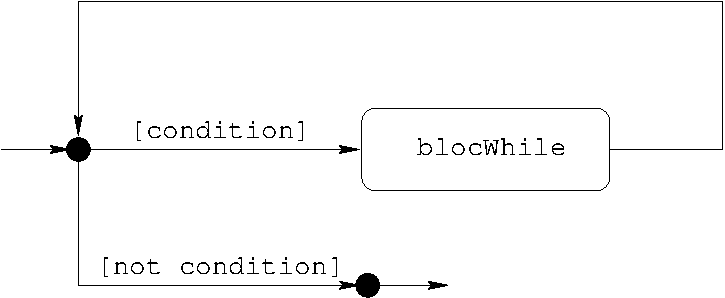
\includegraphics[width=9cm]{../fig/uml4.pdf}$$

\end{frame}
\note{
\mbox{}\null\vfill

\begin{td}[Fonction exponentielle]
Ecrire un algorithme qui calcule $\exp(x)$
en fonction de son d\'eveloppement en série entière. 
$$\displaystyle y = \exp(x) \approx \sum_{k=0}^{n} u_k = \sum_{k=0}^{n} \frac{x^{k}}{k!} = 
	1 + x + \frac{x^2}{2} + \ldots + \frac{x^{n}}{n!}$$
Les calculs seront arr\^et\'es lorsque la valeur absolue du terme $u_k$ sera inf\'erieure 
\`a un certain seuil $s$ ($0 < s < 1$). On n'utilisera ni la fonction {\em puissance} ($x^n$) 
ni la fonction {\em facto\-riel\-le} ($n!$) pour effectuer le calcul de $\exp(x)$.
\end{td}
}
%------------------------------------------



%------------------------------------------
\begin{frame}
\frametitle{\uppercase{Boucles}}
\framesubtitle{\uppercase{Parcours de séquence}}
%------------------------------------------
\begin{block}{Boucle {\tt for}}
$$\fbox{\begin{minipage}{9cm}\tt 
\alert{for} element \alert{in} sequence\alert{:} bloc
\end{minipage}}$$

La séquence peut être 
\begin{itemize}
\item une séquence explicite

	Exemples : {\tt [5,6,7]},%\pause {\tt [3,-2,0,1]},%\pause {\tt ["a","b"]}
%\pause
\item une séquence calculée ({\tt range(min,max,pas)})

	Exemples : \begin{tabular}[t]{l@{$\rightarrow$}l}
	{\tt range(0,5,2)} & {\tt [0,2,4]} \\%\pause
	{\tt range(0,3,1)} & {\tt [0,1,2]} \\%\pause
	{\tt range(0,3)} & {\tt [0,1,2]} \\%\pause
	{\tt range(3)} & {\tt [0,1,2]}
	\end{tabular}
\end{itemize}
\end{block}

\end{frame}
\note{
{\bf Définitions}\begin{description}
\item[séquence] suite ordonnée d'éléments, éventuellement vide, 
accessibles par leur rang dans la séquence.
\end{description}
\null\vfill

\begin{rem}[Principales opérations sur les séquences en \python]
$$\begin{tabular}{|l|p{7cm}|}
\hline 
{\bf Operation} &	\bf Result 	\\
\hline
\tt x in s      & {\tt True} if an item of {\tt s} is equal to {\tt x}, else {\tt False} \\ 	
\tt x not in s 	& {\tt False} if an item of {\tt s} is equal to {\tt x}, else {\tt True}\\
\hline 	
\tt s1 + s2 	& the concatenation of {\tt s1} and {\tt s2}\\ 	 
\tt s * n, n*s 	& {\tt n} copies of {\tt s} concatenated \\	
%\hline
%\end{tabular}$$
%$$\begin{tabular}{|l|p{9cm}|}
\hline
\tt s[i] 	& {\tt i}'th item of {\tt s}, origin {\tt 0}\\ 	
\tt s[i: j]     & \\
\tt s[i: j:step]& Slice of {\tt s} from {\tt i} (included) to {\tt j}(excluded).\newline
                  Optional {\tt step} value, possibly negative (default: {\tt 1}). \\	
\hline
\tt len(s) 	& Length of s \\	 
\tt min(s) 	& Smallest item of s \\	
\tt max(s) 	& Largest item of s \\
\hline
\end{tabular}$$
\end{rem}
}
%------------------------------------------

%------------------------------------------
\begin{frame}
\frametitle{\uppercase{Parcours de séquence}}
\framesubtitle{\uppercase{Affichage élément par élément}}
%------------------------------------------
\begin{columns}\tt
\column{5.25cm}
\fbox{\begin{minipage}{5.75cm}\color{blue}
s = [6,7,8,9,10]\\
{\color{black}print(s)}\\
\alert{for} e \alert{in} s\alert{:}\\
\mbox{}\ \ print(e)\\
{\color{black}print(s)}
\end{minipage}}
%\pause

\column{5.25cm}
$$\begin{array}{|c|c|}
\hline
s & e \\
\hline
\mbox{}[6,7,8,9,10] & \\\hline
%\pause
  & 6 \\%\pause
  & 7\\%\pause
  & 8\\%\pause
  & 9\\%\pause
  & 10\\\hline
%\pause
\mbox{}[6,7,8,9,10] & \\
\hline
\end{array}$$

\end{columns}

\end{frame}
\note{
\mbox{}\null\vfill

\begin{td}[Affichage inverse]
Ecrire un algorithme qui affiche les caractères d'une séquence {\tt s},
un par ligne en partant de la fin de la séquence.
\end{td}
}
%------------------------------------------

%------------------------------------------
\begin{frame}
\frametitle{\uppercase{Parcours de séquence}}
\framesubtitle{\uppercase{Somme arithmétique}}
%------------------------------------------
$$s = \sum_{i=1}^{i=n} i$$

\begin{columns}\tt
\column{5.25cm}
\fbox{\begin{minipage}{5.25cm}\color{blue}
n = 4\\
s = 0\\
{\color{black}print(n, i, s)}\\
\alert{for} i \alert{in} range(1,n+1)\alert{:}\\
\mbox{}\ \ s = s + i\\
\mbox{}\ \ {\color{black}print(n, i, s)}\\
{\color{black}print(n, i, s)}
\end{minipage}}
%\pause

\column{5.25cm}
$$\begin{array}{|c|c|r|}
\hline
n & i & s \\
\hline
4 & ? & 0 \\\hline
%\pause
4 & 1 & 1 \\%\pause
4 & 2 & 3 \\%\pause
4 & 3 & 6 \\%\pause
4 & 4 & 10 \\\hline
%\pause
4 & 4 & 10 \\
\hline
\end{array}$$
$$s = 1 + 2 + 3 + 4 = 10 = \sum_{i=1}^{i=4} i$$

\end{columns}

\end{frame}
\note{
\mbox{}\null\vfill

}
%------------------------------------------


%------------------------------------------
\begin{frame}<presentation>
\frametitle{\uppercase{Parcours de séquence}}
\framesubtitle{\uppercase{Factorielle}}
%------------------------------------------
$$f = n! = \prod_{i=1}^{i=n} i$$

\begin{columns}\tt
\column{5.25cm}
\fbox{\begin{minipage}{5.25cm}\color{blue}
n = 4\\
f = 1\\
{\color{black}print(n, i, f)}\\
\alert{for} i \alert{in} range(1,n+1)\alert{:}\\
\mbox{}\ \ f = f * i\\
\mbox{}\ \ {\color{black}print(n, i, f)}\\
{\color{black}print(n, i, f)}
\end{minipage}}
%\pause

\column{5.25cm}
$$\begin{array}{|c|c|r|}
\hline
n & i & f \\
\hline
4 & ? & 1 \\\hline
%\pause
4 & 1 & 1 \\%\pause
4 & 2 & 2 \\%\pause
4 & 3 & 6 \\%\pause
4 & 4 & 24 \\\hline
%\pause
4 & 4 & 24 \\
\hline
\end{array}$$
$$s = 1 \cdot 2 \cdot 3 \cdot 4 = 24 = \prod_{i=1}^{i=4} i$$

\end{columns}

\end{frame}
\note{
\mbox{}\null\vfill

\begin{td}[Itérations imbriquées]
Qu'affichent les itérations suivantes ?
\begin{enumerate}
\item 
	{\footnotesize\tt
	for i in range(1,10):\\
	\mbox{}\ \ for j in range(0,11) :\\
	\mbox{}\ \ \ \ print(i, 'x', j, ' = ', i*j)\\
	\mbox{}\ \ print()
	}
\item 
	{\footnotesize\tt
	for n in range(10) :\\
  	\mbox{}\ \ for p in range(n+1) :\\
    	\mbox{}\ \ \ \ num = 1\\
    	\mbox{}\ \ \ \ den = 1\\
    	\mbox{}\ \ \ \ for i in range(1,p+1) :\\
      	\mbox{}\ \ \ \ \ \ num = num*(n-i+1)\\
      	\mbox{}\ \ \ \ \ \ den = den*i\\
    	\mbox{}\ \ \ \ c = num/den\\
    	\mbox{}\ \ \ \ print(c,end=' ')\\
  	\mbox{}\ \ print()
	}
\end{enumerate}
\end{td}
}


%------------------------------------------


%------------------------------------------
\begin{frame}<presentation>
\frametitle{\uppercase{Boucles}}
\framesubtitle{\uppercase{Parcours de séquence}}
%------------------------------------------
Boucle {\tt for}
$$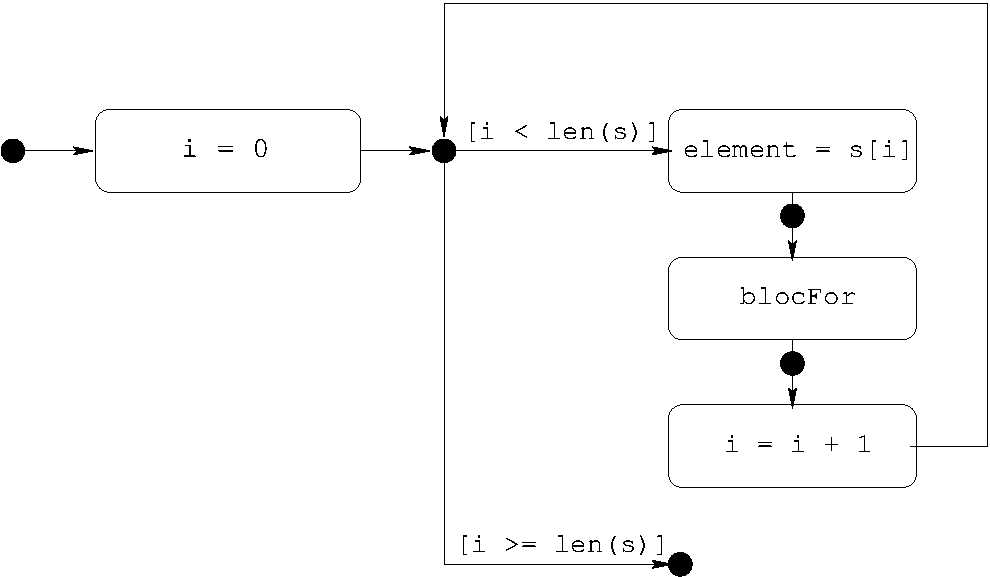
\includegraphics[width=9cm]{../fig/uml7.pdf}$$

\end{frame}
\note{
\mbox{}\null\vfill

\begin{td}[Nid d'abeilles]
Ecrire un algorithmequi dessine un nid d'abeilles formé
de $n\times m$ hexagones en quinconce comme sur la figure 
ci-dessous.

\centerline{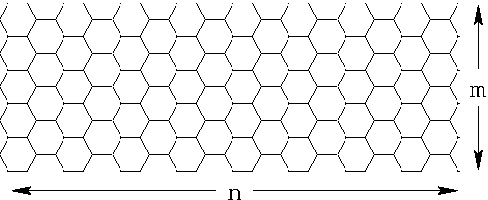
\includegraphics[width=6cm]{../fig/motif.pdf}}
\end{td}

}
%------------------------------------------


%------------------------------------------
\begin{frame}<presentation>
\frametitle{\uppercase{Boucles}}
\framesubtitle{\uppercase{Equivalence boucles {\tt for} et {\tt while}}}
%------------------------------------------
\begin{columns}[T]
\column{5.25cm}
\framebox{\begin{minipage}{5.25cm}\small\tt\color{blue}
\alert{for} i \alert{in} range(min,max,pas)\alert{:}\\
\mbox{}\ \ {\color{black}bloc}
\end{minipage}}
%\pause

$$\begin{minipage}{5.25cm}\tt
{\small\# élévation à la puissance}\\
\mbox{}\\
p = 1\\
\alert{for} i \alert{in} range(n)\alert{:}\\
\mbox{}\ \ p = p * x
\end{minipage}$$

%\pause
\column{5.25cm}
\framebox{\begin{minipage}{5.25cm}\small\tt\color{blue}
i = min\\
\alert{while} i < max\alert{:}\\
\mbox{}\ \ {\color{black}bloc}\\
\mbox{}\ \ i = i + pas
\end{minipage}}
%\pause

$$\begin{minipage}{5.25cm}\tt
p = 1\\
i = 0\\
\alert{while} i < n\alert{:} \\
\mbox{}\ \ p = p * x\\
\mbox{}\ \ i = i + 1
\end{minipage}$$

\end{columns}

\end{frame}
\note{
\mbox{}\null\vfill

\begin{td}[Boucles {\tt for} et {\tt while} imbriquées]
Qu'affichent les itérations suivantes ?
\begin{enumerate}
\item
{\footnotesize\tt
for i in range(0,10) :\\
\mbox{}\ \ j = 10 - i\\
\mbox{}\ \ while j > 0 :\\
\mbox{}\ \ \ \ print('*',end=' ')\\
\mbox{}\ \ \ \ j = j - 1\\
\mbox{}\ \ print()
}
\item
{\footnotesize\tt
n = 0\\
while n < 10 :\\
\mbox{}\ \ for p in range(n+1) :\\
\mbox{}\ \ \ \ num = 1\\
\mbox{}\ \ \ \ den = 1\\
\mbox{}\ \ \ \ for i in range(1,p+1) :\\
\mbox{}\ \ \ \ \ \ num = num*(n-i+1)\\
\mbox{}\ \ \ \ \ \ den = den*i\\
\mbox{}\ \ \ \ c = num/den\\
\mbox{}\ \ \ \ print(c,end=' ')\\
\mbox{}\ \ print()\\
\mbox{}\ \ n = n + 1
}
\end{enumerate}
\end{td}
}
%------------------------------------------

%------------------------------------------
\begin{frame}<presentation>
\frametitle{\uppercase{Boucles}}
\framesubtitle{\uppercase{Equivalence boucles {\tt for} et {\tt while}}}
%------------------------------------------
\begin{columns}[T]
\column{5.25cm}
\framebox{\begin{minipage}{5.25cm}\small\tt\color{blue}
\alert{for} element \alert{in} sequence\alert{:}\\
\mbox{}\ \ {\color{black}bloc}
\end{minipage}}
%\pause

$$\begin{minipage}{5.25cm}\tt
\# affichage élément \\
\# par élément\\
\mbox{}\\
s = [6,7,8,9,10]\\
{print(s)}\\
\alert{for} e \alert{in} s\alert{:}\\
\mbox{}\ \ print(e)\\
{print(s)}
\end{minipage}$$

%\pause
\column{5.25cm}
\framebox{\begin{minipage}{5.25cm}\small\tt\color{blue}
i = 0\\
\alert{while} i < len(sequence)\alert{:}\\
\mbox{}\ \ element = sequence[i]\\
\mbox{}\ \ {\color{black}bloc}\\
\mbox{}\ \ i = i + 1
\end{minipage}}
%\pause

$$\begin{minipage}{5.25cm}\tt
s = [6,7,8,9,10]\\
{print(s)}\\
i = 0\\
\alert{while} i < len(s)\alert{:}\\
\mbox{}\ \ e = s[i]\\
\mbox{}\ \ print(e)\\
\mbox{}\ \ i = i + 1\\
{print(s)}
\end{minipage}$$

\end{columns}

\end{frame}
\note{}
%-------------------------------------------------------------------------
\end{document}
%-------------------------------------------------------------------------
